\documentclass[sigconf]{acmart}
\AtBeginDocument{%
  \providecommand\BibTeX{{%
    Bib\TeX}}}
\usepackage{siunitx}
\usepackage{bm}
\settopmatter{printacmref=false}
\setcopyright{none}

\begin{document}

\title{In Silico Model of Tumor Diagnosis based on Bloodstream Penetrating Extracellular Vesicles}
\author{Robin Brendel}
\email{robin.brendel@student.uni-luebeck.de}
\affiliation{%
  \institution{University of Lübeck}
  \state{Schleswig-Holstein}
  \country{Germany}
}

\begin{abstract}
Extracellular vesicles (EVs) have drawn a lot of scientific attention in the last ten years as natural drug carriers and disease biomarkers, particularly for cancer. Although a few studies have monitored tumor-derived EVs in the bloodstream or extracellular spaces, none have fully modeled their concurrent passage through surrounding tissues, blood vessels, and tumor microenvironments. We created an in silico computer model that replicates the entire procedure. Our model includes EV release from cancer cells, circulation through arterial-capillary-venous networks, transport across tissue, and eventual bloodstream entry. Based on the speed at which tumor EVs enter the bloodstream, we suggest a novel diagnostic approach for sub-millimeter tumors by examining simulation results. Our results highlight the method's sensitivity to tumor size and its potential for non-invasive cancer detection. 
\end{abstract}

\keywords{In Silico, Extracellular Vesicles, COMSOL, Tumor, Diagnosis, Cancer, Biomarkers}

\maketitle

\section{Introduction}
\label{sec: introduction}
Extracellular vesicles (EVs) are tiny lipid-bound particles (30 nm to \SI{5}{\micro\meter}) released by cells into their surroundings \cite{Doyle_2019}. Their lipid walls protect contents from enzymes and help cross biological barriers \cite{Arjmandi_2021}. Combining durability, natural targeting, and cargo-specificity, EVs offer exciting potential as diagnostic biomarkers and natural drug delivery vehicles, particularly for cancer \cite{Doyle_2019}.

EVs don't move locally. They can enter the bloodstream and travel systemically with the blood flow. This enables non-invasive diagnostics, prompting mathematical models of EV blood propagation \cite{Ferguson_2020}. Understanding this tissue-blood journey is crucial for improving diagnostics and drug delivery. For an overview of these mechanisms the following paper is given \cite{Sykov__2008}. Beyond expensive invasive studies in vivo or limited experiments in vitro, computer models provide cost-effective in silico alternatives that can show complex biological processes while reducing experiments in the lab. 

Our paper is structured as follows: In the second section we explain our system model for the tissue and blood vessels network. After that, in section three we summarize findings and outline future work.

\section{Design and Results}
\label{sec: design-results}

\subsection{System Model}
\label{subsec: sys-model}
Figure 1 shows our realistic biological scenario with the following distinct zones: artery (blood inlet), vein (blood outlet), capillary network ($\Omega_{\text{c}}$), tumor area ($\Omega_{\text{t}}$), and healthy tissue ($\Omega_{\text{h}}$). Since tumors need oxygen and nutrients, capillaries infiltrate cancerous regions. Tumor-generated EVs can either penetrate capillary walls into blood or migrate into healthy tissue. The bloodstream entry rate depends on vessel wall permeability which is modeled by:
\begin{equation}
  k_{\mathrm{p}}=\frac{D_{\mathrm{w}}}{d_{\mathrm{w}}}
\end{equation}

where $D_{\mathrm{w}}$ is the EV diffusion coefficient within the wall and $d_{\mathrm{w}}$ is wall thickness, which parameters are listed in \cite{Zoofaghari_2023}. Thin walls of capillaries and high $k_{\mathrm{p}}$ make them primary EV gateways, so we established specialized boundary conditions to model biologically realistic transitions:
\begin{itemize}
  \item Capillary-tissue interface, where a diffusion barrier connects EV flow between tissue ($J_{\text{t}}$/$J_{\text{h}}$) and blood ($J_{\text{c}}$) to concentration differences ($c_{\text{t}}$/$c_{\text{h}}$ vs. $c_{\text{c}}$). According to diffusion principles, EVs flow from regions of higher to lower concentration.
  \item Tumor-healthy interface, where a partition condition ($c_{\text{h}} = k_{\text{t}}c_{\text{t}}$) governs EV migration, with $k_{\text{t}} = \sqrt{D_{\text{t}}/D_{\text{h}}}$ that depends on diffusion differences.
  \item Healthy tissue boundary, where partially absorbing condition models EV uptake.
\end{itemize}
EVs primarily drift with blood flow  ($\bm{u}_{\text{b}}$) as soon as they are in the blood system. Changes in EV concentration in capillaries, tumors, and healthy tissue are described by advection-diffusion equations, which take into consideration flow drift, diffusion, degradation, and release rates ($R_{\text{t}}$, $R_{\text{h}}$). Navier-Stokes equations were used to model blood flow as laminar flow. The EV penetration rate into circulation ($R_{\text{s}}$, mol/s), which was determined by integrating EV flux across venule cross sections (VCS), was the primary diagnostic metric:

\begin{equation}
  R_{\text{s}}=\iint_{\text{VCS}}c(r,t)u_{n}(r,t)\,\mathrm{d}s
\end{equation}
where $c(r,t)$ describes the concentration differences of EVs and $u_{n}(r,t)$ the blood velocity vertical to the VCS.

\begin{figure}[h]
  \centering
  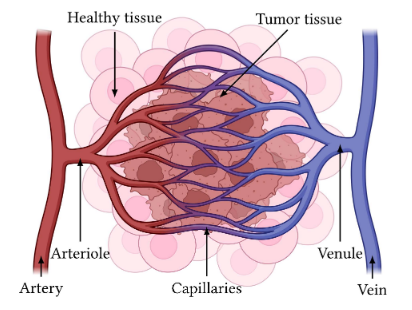
\includegraphics[width=\linewidth]{pictures/schematic_bloodvessels.png}
  \caption{This schematic shows the blood vessels system in healthy and cancerous tissue \cite{Zoofaghari_2023}.}
  \Description{}
\end{figure}

\newpage

\subsection{Results}
\label{sec: num-results}
Our computational framework used COMSOL Multiphysics to solve the relevant equations with finite element methods. The Transport of Diluted Species module captured how EVs move, while the Single-Phase Flow module simulated blood flow. Blood velocity profiles from these flow simulations directly fed into EV transport calculations, with the parameters listed in \cite{Zoofaghari_2023}.

The simulations provided key insights into how EVs interact with tumors and the bloodstream. In tumor regions, we observed a strong buildup of EVs due to dense tissue structure and lower diffusion rates. This effect led to concentration gradients that were 3.5 times higher than those in healthy tissue. That creates strong obstacles for capillary access even when the tissues were close together.

The main results are summarized as follows:
\begin{itemize}
  \item Because the capillary network has a larger total  sectional area than the arteriole and venule, blood flow simulations reveal that the capillary network's velocity components are substantially lower. EV exchange is facilitated by this slow flow.
  
  \item Only a small percentage of EVs diffuse into capillaries, with the majority accumulating in tumor areas. After entering the capillaries, EVs are swiftly transported into the venule and exit the body, where their concentrations rapidly decrease.
  
  \item In order to support efficient clearance through circulation, EV transport streamlines verify that flux is directed toward the vein and intensifies as it approaches the outlet.
  
  \item By examining tumors of different sub-millimeter sizes, the model's diagnostic sensitivity was evaluated:
  \begin{enumerate}
    \item Small tumors produce low EV release rates and the accumulation is localized with limited vascular penetration.
    \item Moderate tumors show increased EV diffusion into capillaries and hence elevated venous EV concentrations.
    \item Large tumors boost EV penetration rate into the bloodstream, with a marked increase in venous flux and concentration.
  \end{enumerate}
  
  \item The EV penetration rate \( R_s \) (mol/s), that is calculated over the venule cross section, demonstrates a clear dependence on tumor size and blood flow parameters. This relationship supports the viability of EV-based diagnostics for detecting early-stage, sub-millimeter tumors.

  \item Uniform EV size was assumed in this model to eliminate the effects of diffusion dispersion and focus solely on transport and accumulation dynamics.
\end{itemize}


\section{Conclusion}
\label{sec: conclusion}
This study presents a computational framework for modeling how EVs move from tumor tissue into the bloodstream. The goal is to evaluate the possibility of using EV-based liquid biopsies for early cancer detection. By combining advection-diffusion dynamics with microvascular blood flow in a realistic tumor-vessel setup, we measured EV accumulation and transvascular penetration across different tumor sizes.

Our results show that even very small tumors can produce detectable EV levels in the venous outflow, as long as enough transvascular transport occurs. The simulations reveal a nonlinear increase in venous EV concentration with tumor size, highlighting its sensitivity to early-stage tumor development. Additionally, the model identifies key physical mechanisms, like capillary slowing, pressure-driven flow, and diffusion limitations, that influence EV distribution and clearance.

These findings support the idea of using EV concentration measurements in venous blood as a less invasive method for early tumor detection. The modeling framework provides a basis for refining diagnostic thresholds and improving sampling strategies in future experimental and clinical studies. Further work may build on this model by including varying tumor properties, different EV sizes, and dynamic systemic clearance to enhance biological realism.


\bibliographystyle{ACM-Reference-Format}
\bibliography{my_library}

\appendix

\section{About this paper}
This paper is a summary of an original source paper. The source paper with the same title you can find in \cite{Zoofaghari_2023}

\end{document}
\endinput